\section{Results}
{\bf copy/ paste from email May 9 by Nick}

{\bf Q. 2.}  I don't quite get what is the accuracy you are reporting on the first Figure. Why does it make sense to look at the best-performing task ? 

my initial fiddling with these data was aimed at finding the task pair that gives most reliable classification for a given user (so they can use those tasks to control software etc). so, the best-performing task (maximum classification accuracy) is the task we would select if we're trying to achieve best performance for that subject. my question this time arond was -- to what extent can we degrade (compress) a classification task that does very well before it no longer does very well?

    By the way, I generated the average classification performance per subject directly in the spreadsheet. In most cases, we see little decrease in performance vs. bins. Although the accuracy is always above gambling (50\%), some subjects are clearly harder to classify than others. This is maybe an interesting result to discuss further.


definitely. there's a lot of work on "BCI illiteracy". however, if 67\% is the canonical threshold for acceptable bci, none of our subjects exhibit BCI illiteracy!
 
\begin{figure}
\begin{center}
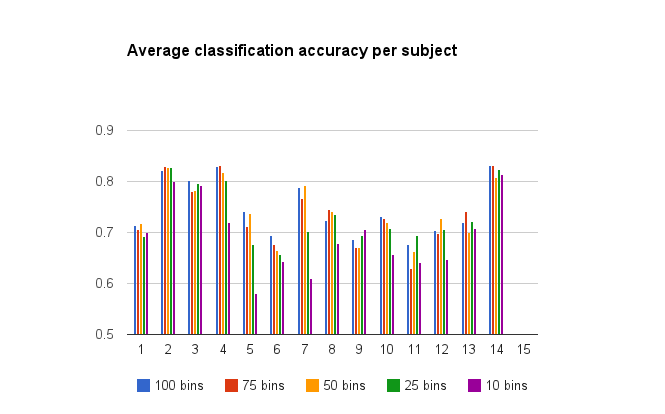
\includegraphics[width=6in]{Figures/avg_classification_accuracy_per_subject.png}
\caption{ }
\label{ }
\end{center}
\end{figure}


i'm wondering if there are a few outlier tasks here - like, a few tasks on which we get very low classification accuracy, dragging down the average
 

{\bf Q. 3.} Related to the average classification accuracy per task pair (second Figure), the difference between task pairs is striking. It seems that all pairs involving "color" rate high, as well as "finger" and "base". However, it's hard to distinguish between "finger" and "base" ! I recall that the "color" task is longer than others. I guess it can be a reason for this result. I attached an updated chart with all x-axis labels.

\begin{figure}
\begin{center}
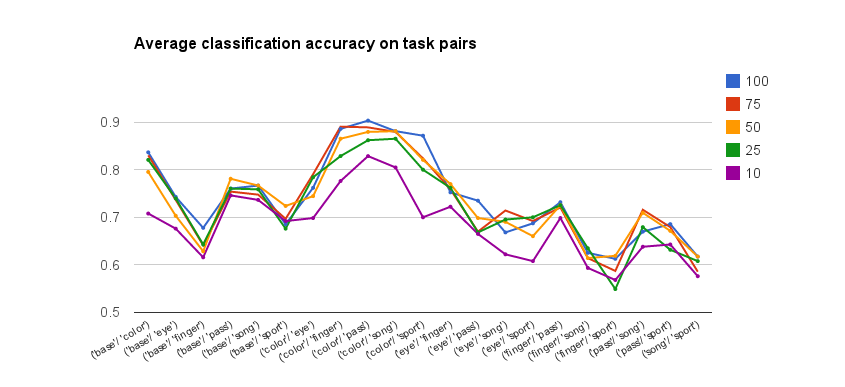
\includegraphics[width=6in]{Figures/avg_classification_accuracy_taskpairs.png}
\caption{ }
\label{ }
\end{center}
\end{figure}

{\bf Q. 4.} Overall, I agree that for bins = [100,75,50,25] there is little difference. However, bin = 10 is clearly less good.


definitely. one interesting question is - why is ten suddenly bad when 25 is fine? is there some way to predict what bin size will start to behave poorly? some way that's derived from principals about the ML itself, rather than trial and error
 


{\bf Q. 5.} I also recall that we have discussed that it would be great to look how long (in seconds) it take to properly classify. Concretely, we have more or less 10 seconds per sample (at the exception of the "color" task as far as I remember). So instead of classifying on the binned probability density function (pdf) build from an averaging power spectra over 10 seconds, what happens if we classify based on pdfs built on averaging power spectra on 1,2,3,...., and then 10 seconds instead ?

 
i am interested in this question too....... when we someday have an elegant online data collection pipeline, we might be able to answer this question easily and in a fun way